\documentclass[twoside,a4wide,11pt]{article}\usepackage[]{graphicx}\usepackage[]{color}
%% maxwidth is the original width if it is less than linewidth
%% otherwise use linewidth (to make sure the graphics do not exceed the margin)
\makeatletter
\def\maxwidth{ %
  \ifdim\Gin@nat@width>\linewidth
    \linewidth
  \else
    \Gin@nat@width
  \fi
}
\makeatother

\definecolor{fgcolor}{rgb}{0.345, 0.345, 0.345}
\newcommand{\hlnum}[1]{\textcolor[rgb]{0.686,0.059,0.569}{#1}}%
\newcommand{\hlstr}[1]{\textcolor[rgb]{0.192,0.494,0.8}{#1}}%
\newcommand{\hlcom}[1]{\textcolor[rgb]{0.678,0.584,0.686}{\textit{#1}}}%
\newcommand{\hlopt}[1]{\textcolor[rgb]{0,0,0}{#1}}%
\newcommand{\hlstd}[1]{\textcolor[rgb]{0.345,0.345,0.345}{#1}}%
\newcommand{\hlkwa}[1]{\textcolor[rgb]{0.161,0.373,0.58}{\textbf{#1}}}%
\newcommand{\hlkwb}[1]{\textcolor[rgb]{0.69,0.353,0.396}{#1}}%
\newcommand{\hlkwc}[1]{\textcolor[rgb]{0.333,0.667,0.333}{#1}}%
\newcommand{\hlkwd}[1]{\textcolor[rgb]{0.737,0.353,0.396}{\textbf{#1}}}%
\let\hlipl\hlkwb

\usepackage{framed}
\makeatletter
\newenvironment{kframe}{%
 \def\at@end@of@kframe{}%
 \ifinner\ifhmode%
  \def\at@end@of@kframe{\end{minipage}}%
  \begin{minipage}{\columnwidth}%
 \fi\fi%
 \def\FrameCommand##1{\hskip\@totalleftmargin \hskip-\fboxsep
 \colorbox{shadecolor}{##1}\hskip-\fboxsep
     % There is no \\@totalrightmargin, so:
     \hskip-\linewidth \hskip-\@totalleftmargin \hskip\columnwidth}%
 \MakeFramed {\advance\hsize-\width
   \@totalleftmargin\z@ \linewidth\hsize
   \@setminipage}}%
 {\par\unskip\endMakeFramed%
 \at@end@of@kframe}
\makeatother

\definecolor{shadecolor}{rgb}{.97, .97, .97}
\definecolor{messagecolor}{rgb}{0, 0, 0}
\definecolor{warningcolor}{rgb}{1, 0, 1}
\definecolor{errorcolor}{rgb}{1, 0, 0}
\newenvironment{knitrout}{}{} % an empty environment to be redefined in TeX

\usepackage{alltt}
\usepackage[left=2.5cm,top=2cm,right=2cm,bottom=2.5cm,bindingoffset=0.5cm]{geometry}
\usepackage{amsmath} 
\usepackage[affil-it]{authblk}
\usepackage{hyperref}
\usepackage{fullpage}
\usepackage{pdflscape}
\usepackage[backend=bibtex,sorting=none,style=ieee]{biblatex}
\usepackage{setspace}
\usepackage{inconsolata}
\bibliography{chromothripsis}

\title{Shatterseek: an R package for the detection of chromothripsis from Next-Generation Sequencing (NGS) data}
%structural rearrangements and copy number data

\author[1,2,3]{\rm Isidro Cortes-Ciriano}%\thanks{isidrolauscher@gmail.com}} 
\author[4]{\rm Ruibin Xi}%\thanks{ruibinxi@math.pku.edu.cn}}
\author[1,2]{\rm Peter J. Park\thanks{peter\_park@hms.harvard.edu}}

\affil[1]{Department of Biomedical Informatics, Harvard Medical School, Boston, Massachusetts, USA}
\affil[2]{Ludwig Center at Harvard, Boston, MA 02115, USA}
\affil[3]{Centre for Molecular Science Informatics, Department of Chemistry, University of Cambridge, Lensfield Road, Cambridge CB2 1EW, United Kingdom}
\affil[4]{School of Mathematical Sciences and Center for Statistical Science, Peking University, Beijing 100871, China}
\setlength{\parindent}{0pt}
\setlength{\parskip}{\baselineskip}

%--------------------------------------------------------------------------------
\IfFileExists{upquote.sty}{\usepackage{upquote}}{}
\begin{document}
%--------------------------------------------------------------------------------
\maketitle
\tableofcontents
\onehalfspacing

%-------------------------
\section{Introduction} %from Next-Generation Sequencing (NGS) data}
%-------------------------
Chromothripsis refers to the genomic alterations characterized by massive de novo rearrangements, 
often generated in a single catastrophic event, where the DNA is shattered into a number of 
fragments that are subsequently stitched together in random order and orientation. 
Chromothripsis can be confined to small chromosomal regions or can affect multiple chromosomes,
and can involve from tens to hundreds of rearrangements \cite{Stephens2011}.
Therefore, chromothripsis represents a mechanism for the accrual of tens to hundreds of rearrangements in a few cell divisions.\\
\\
Chromothripsis regions are characterized by copy number profiles oscillating between two or three states,
(in cases where partial duplications follow chromothripsis), 
interspersed loss of heterozygosity (LOH), and clusters of interleaved SVs, 
where the proportions of fragment joins (i.e., duplication-like, deletion-like, head-to-head and tail-to-tail inversions) are roughly equal, consistent with the random stitching of genomic fragments through mostly non-homologous end-joining (NHEJ) DNA repair.\\
\\
Initial studies used array-derived copy number profiles to detect chromothripsis, 
as the amount of whole-genome sequencing data sets was limited \cite{Kim2013,Cai2014}.
%thus preventing to 
SNP arrays do not permit to fully characterize the genome-wide landscape of structural rearrangements at
single-base resolution.
%and hence,characterize the types of SVs comprised in regions subject to chromothripsis.
Nevertheless, the detection of chromothripsis is more accurate  
if structural rearrangements and copy number data are integrated \cite{Notta2016,Li2014,Korbel2013,Govind2014}.
The increasing amount of whole-genome sequencing data sets 
thus requires the development of easy-to-use pipelines to detect chromothripsis from NGS data.
%These studies have contributed to better characterize the landscape and rates of chromothripsis across human cancers.
Korbel and Campbell \cite{Korbel2013} proposed a set of statistical criteria for the detection of chromothripsis that have been widely used in the literature. 
There exist two publicly available packages for the detection of chromothripsis, namely: 
CTLP scanner \cite{Cai2014,Yang2016} and Shatterproof \cite{Govind2014}.
The former uses SNP array data, whereas the latter CN and SV data.\\
\\
We have developed Shatterseek, an R package that integrates copy number and SV data for the detection and 
visualization of chromothripsis events from NGS data.
Shatterseek implements a custom grpah-based approach to identify candidate chromothripsis regions, 
and then applies a set of statistical criteria based on Korbel and Campbell \cite{Korbel2013}
to detect both intra- and interchromosomal chromothripsis events.
In addition, Shatterseek provides functionalities for the easy visualization of SVs, as well as CN and LOH profiles.
Visual inspection of candidate chromothripsis regions is still required in a number of cases due to the complexity of the observed events, and the overlapping features of chromothripsis and other complex events.
% Shatterseek was validated using experimental daa
% comparison Shatterproof
We have recently validated Shatterseek in a large-scale
study of ca. 2,600 cancer genomes and its higher performance with respect to Shatterproof.
We refer the reader to this work for further details about the rates and characteristics of chromothripsis across diverse human cancers.
The chromothripsis calls for all these tumors generated using Shatterseek can be accessed at 
http://compbio.med.harvard.edu/chromothripsis/ \\
\\
In the next sections, we explain in detail the statistical criteria implemented in Shatterseek to detect
chromothripsis events,
and illustrate its functionalities using data from X cancer patients.

%-------------------------
\section{Workflow implemented in Shatterseek}
%-------------------------
To identify chromothripsis-like patterns in cancer genomes, we implemented and extended 
the set of  criteria proposed by Campbell and Korbel \cite{Korbel2013}. 
The pipeline to detect chromothripsis consists of three major steps, namely:
(i) discovery of clusters of interleaved SVs using a graph-based approach,
(ii) evaluation of a set of statistical criteria in the genomic regions spanned by these clusters,
and (iii) evaluation of whether chromothripsis is confined to a single or to multiple chromosomes.\\
\\

\begin{figure}[htb]
\begin{center}
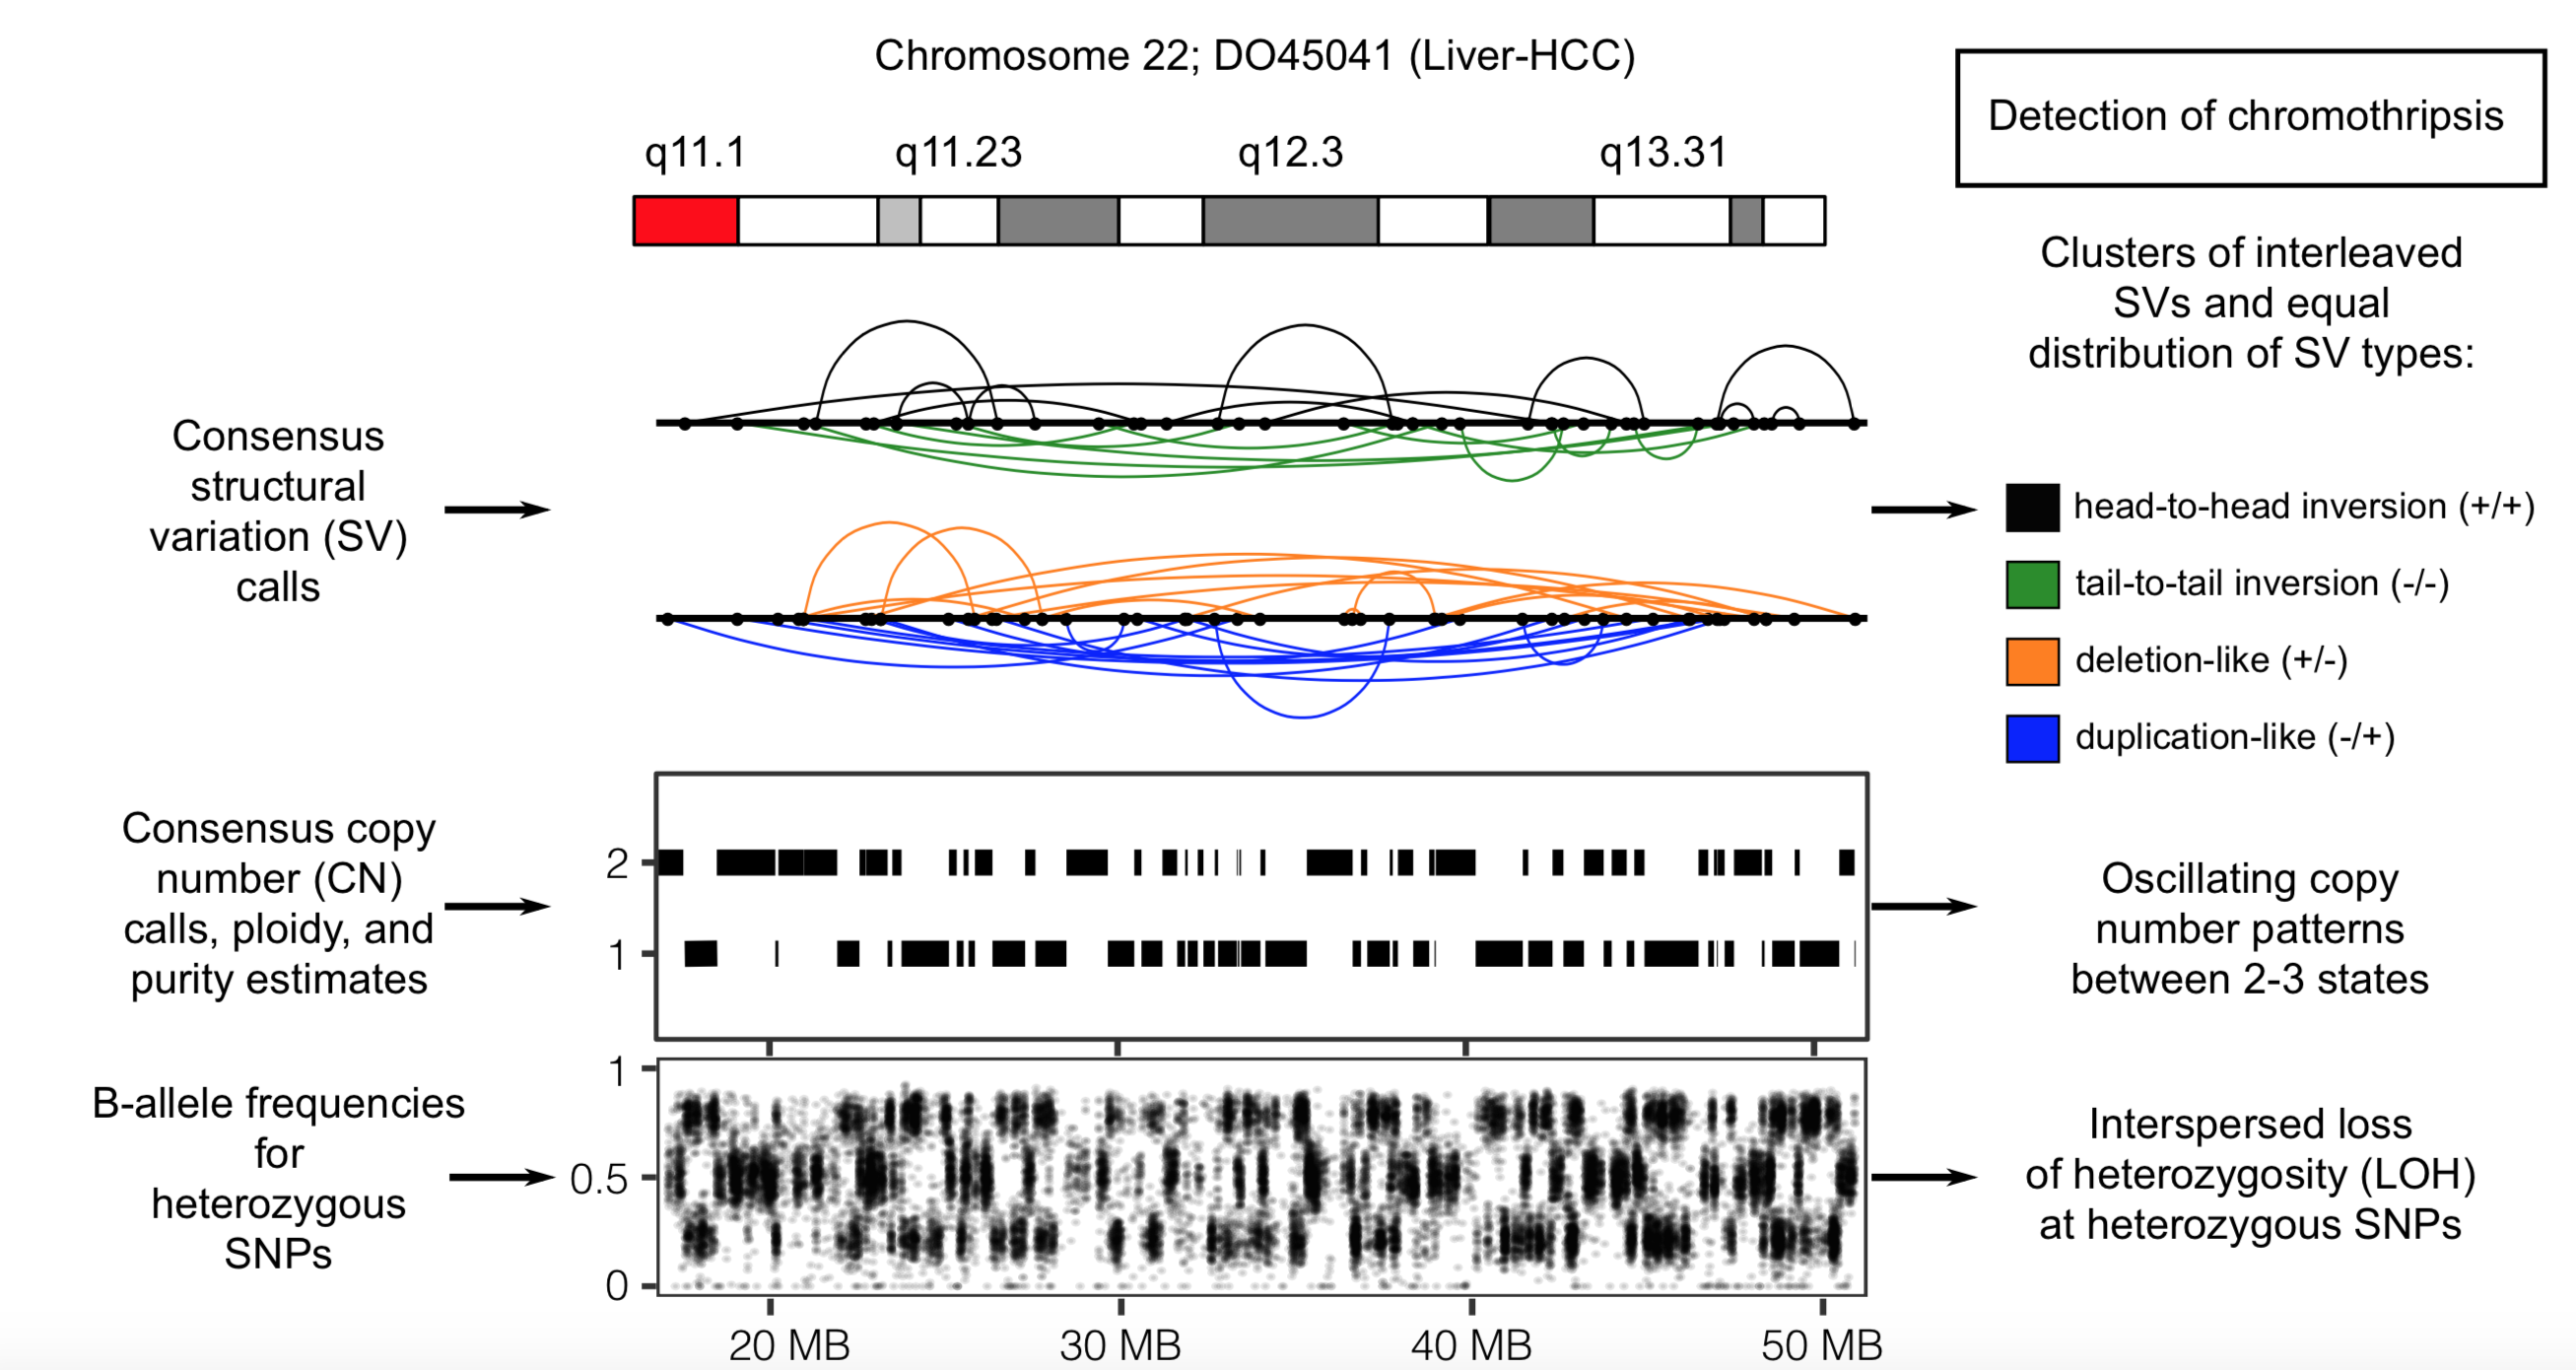
\includegraphics[width=\textwidth]{workflow_tutorial.png}
\caption{ssdfT}
\end{center}
\end{figure}

\subsection{Detection of clusters of interleaved SVs}

Given that chromothripsis events generate clusters of interleaved rearrangements, 
we firstly scanned the cancer genomes for the presence of clusters of interleaved SVs.
We consider that two SVs are interleaved if the genomic regions bridged by their breakpoints overlap but are not nested. 
To find clusters within a given chromosome, 
Shatterseek constructs an undirected graph using intrachromosomal SVs 
whose nodes correspond to SVs and whose edges connect interleaved SVs. 
Thus, clusters of SVs can be detected by finding the connected components in the graph. 
The connected component in each chromosome with the highest number of SVs is considered for further analysis. 
By default, Shatterseek only considers chromosomes 1-22 and X.
In the following, we use the term {\it chromothripsis region} to refer to the genomic regions affected by chromothripsis within one chromosome, whereas we term {\it chromothripsis event} the set of chromothripsis regions involved in a single catastrophic event.
Thus, a chromothripsis event can affect a single chromosome, multiple regions within a chromosome, or comprise genomic regions from multiple chromosomes.

\subsection{Statistical criteria implemented in Shatterseek}

Once the clusters of interleaved SVs are detected, Shatterseek evaluates the following statistical criteria based on the work by Korbel and Campbell \cite{Korbel2013}.

% We decided to only consider the criteria of loss of heterozygosity proposed by (Korbel and Campbell, 2013) when examining the set of canonical chromothripsis calls detected in diploid genomes. We did not consider this criterion to call chromothripsis across the entire tumor cohort because we noticed that some bona fide chromothripsis cases identified in low-purity samples (e.g., Figure 2c) might not meet the cut-off for statistical significance due to the infiltration of normal tissue. In such a case, the allelic ratios (i.e., B allele frequencies) for heterozygous SNPs would not divert significantly from 0.5, and thus, would hamper the observation of alternating LOH patterns associated to copy losses (Song et al., 2012). This phenomenon is exacerbated when chromothripsis occurs in aneuploid tumors due to increased CN, and hence, chromothripsis events do not necessarily lead to LOH (see e.g., Supplementary Figure 5C).

\subsubsection{Equal distribution of fragment joins}

Once the SV clusters are detected, Shatterseek evaluates whether the distribution of DNA fragment joins,
i.e., deletion-like (+/-; or "head"/"tail"), duplication-like (-/+), head-to-head (+/+), and tail-to-tail (-/-) inversions,
diverges from a multinomial distribution with equal probabilities for each SV category using the goodness-of-fit test for the multinomial distribution using the from the R package stats (chiq.test function).
The types of SVs are determined by the orientation of the reads mapped to the breakpoints (see \cite{Zhang2013} for further details).

\subsubsection{Chromosomal enrichment of breakpoints}
Massive chromothripsis events, which involve hundreds of SVs,
generally affect entire or multiple chromosomes against the background of 
quiescent genomes.
Thus, in these cases the chromosomes harboring chromothripsis are highly enriched for breakpoints.
An example of a chromothripsis event is depicted in Figure 1.


To test for the enrichment of breakpoints in each chromosome,
Shatterseek uses the binomial test corrected for mappability. 
We note that this test might be misleading for focal chromothripsis events
appearing in highly rearranged genomes, where
other chromosomes not displaying chromothripsis harbor a number of SVs (interleaved or not) comparable to that
detected in chromosomes displaying chromothripsis. 
Therefore, this criterion needs to be interpreted carefully on a per-case basis.

\subsubsection{Random distribution of breakpoints}
Shatterseek also evaluates whether the distribution of the breakpoints comprised the SV clusters
differs from an exponential as described by Korbel and Campbell \cite{Korbel2013}.

\subsubsection{Number of oscillating copy number segments}
A major feature of chromothripsis that can be detected from copy number data is the 
presence of copy number profiles oscillating between two or three copy number states.
This feature has been widely used before to detect chromothripsis from 
genome-wide copy number profiles using operational definitions,
e.g., at least 10 contiguous segments oscillating between two copy number states \cite{Rausch2012}. 

To uncover oscillating patterns in the genomic regions delimited by the distal breakpoints composing 
the clusters of interleaved SVs,
Shatterseek examines whether contiguous genomic segments oscillate between two or three CN states. 

\subsubsection{Interspersed loss of heterozygosity (LOH)}

We decided not to use the criteria of loss of heterozygosity proposed by Campbell and Korbel \cite{Korbel2013}, 
as we noticed that some bona fide chromothripsis cases identified in low-purity samples might not meet this criterion due to the infiltration of normal tissue.
In such a case, the allelic ratios for heterozygous SNPs (i.e., B allele frequencies) would not divert significantly from 0.5, and thus, would hamper the observation of alternating LOH patterns associated to copy losses \cite{Song2012}.
In addition, assessing LOH in aneuploid tumors is often difficult,
where the BAF values for oscillating segments between high CN levels do not vary strongly.\\
\\
However, given that the loss of heterozygosity profiles are very useful to
determine the temporal profile of chromothripsis events, 
and to distinguish chromothripsis from chromoanasynthesis in nearly-diploid cases,
Shatterseek provides capabilities to visualize LOH profiles at chromothripsis regions.
\\

\subsection{Detection of multichromosomal chromothripsis events}
Shatterseek considers that two or more  chromothripsis regions belong to the same 
catastrophic event if these regions +/- 10Kb (default value) are linked by at least two interchromosomal SVs.
Given that the sensitivity of SV detection algorithms is still limited,
it is not always possible to detect rearrangements between all regions belonging to the same chromothripsis event.
Thus, in cases where at least three chromosomes were involved, 
Shatterseek applies transitive reasoning to identify the full extent of the events. 
For instance, if the chromothripsis regions detected in chromosomes 1 and 2 are linked, and those detected in chromosome 2 are also linked to a chromothripsis region in chromosome 3, Shatterseek considers that the chromothripsis patterns detected in these three chromosomes were generated as a result of the same catastrophic event.

% The P values from these three tests were corrected using the FDR method. The level of significance was set to q ≤ 0.2. 
% Finally, the genomic regions delimited by the distal breakpoints composing the clusters of interleaved SVs were further examined for the presence of contiguous genomic segments oscillating between two CN states. 


%-----------------------------------------------------------------------------------------------------
\section{Recommended cut-off values to interpret the output of Shatterseek}

After manual curation of hundreds of massive and focal chromothripsis calls, 
we derived the following guidelines to detect chromothripsis using Shatteseek.

We assign two levels of confidence depending on the set of statistical tests
satisfied by a candidate chromothripsis region.
% consider as high-confidence chromothripsis regions those satisfying at least one of the
% two first sets of cut-off values for the statistical criteria described above:

\begin{itemize}

\item High confidence: at least 6 interleaved intrachromosomal SVs, 7 contiguous segments oscillating between 2 CN states, 
the fragment joins test, and either the chromosomal enrichment or the exponential distribution of breakpoints test.

\item High confidence: at least 3 interleaved intrachromosomal SVs and 4 or more interchromosomal SVs, 7 contiguous segments oscillating between 2 CN states and the fragment joins test.

\item Low confidence: at least 6 interleaved intrachromosomal SVs, 4, 5 or 6 adjacent segments oscillating between 2 CN states, the fragment joins test, and either the chromosomal enrichment or the exponential distribution of breakpoints test.

\end{itemize}

% T(following the criteria previously used )
Application of these criteria to ~2,600 whole genomes still led to a small set of false positives that were removed by visual inspection. 
This is mostly due to the fact that multiple layers of rearragements other than chromothripsis might coexist, and the aggregate of these might satisfy the statistical tests described above.
In addition, chromothripsis regions are highly heterogeneous, running the gamut from massive chromothripsis cases 
invovling hundreds of SVs in an otherwise quiescent genome, 
to focal events in the context of genomes highly rearranged by other mutational processes.
This heterogeneity makes it almost impossible to define a set of criteria with perfect
discriminative power for chromothripsis.
Therefore, we advocate, as far as possible, for the manual curation of candidate chromothripsis regions. 
To facilitate this process, Shatterseek provides functionalities to visually depict the candidate chromothripsis regions. 


%------------------------------------------------------------------------------------------------------
\section{How to use Shatterkeek}
%------------------------------------------------------------------------------------------------------
In the following sections, we illustrate how to install and use Shatterseek to detect and visualize chromothripsis 
using SV and CN data. 
This tutorial assumes minimal knowledge of the R programming language.

\subsection{Installation}
Shatterseek is entirely written in R. 
To install Shatterseek type the following in R: 
\begin{knitrout}
\definecolor{shadecolor}{rgb}{0.969, 0.969, 0.969}\color{fgcolor}\begin{kframe}
\begin{alltt}
\hlkwd{sessionInfo}()
\hlkwd{require}(devtools)
\hlkwd{install_github}(“”)
\end{alltt}
\end{kframe}
\end{knitrout}
Alternatively, please download and install Shatterseek by running in a bash terminal:\\
\begin{knitrout}
\definecolor{shadecolor}{rgb}{0.969, 0.969, 0.969}\color{fgcolor}\begin{kframe}
\begin{alltt}
wget XXXXXXXXXX
R CMD INSTALL shatterSeek_0.4
\end{alltt}
\end{kframe}
\end{knitrout}

\subsection{Load SVs and CN data into R}

XX data from any caller can be used
XX ein PCAWG consensus, etc.. 
XX total copy number in integer format (output of e.g. ASCAT)

We first load Shatterseek and the test data that is provided with the package.
This corresponds to the SV and CN data for a kidney renal cell carcinoma tumor (ICGC ID: DO17373).
\begin{knitrout}
\definecolor{shadecolor}{rgb}{0.969, 0.969, 0.969}\color{fgcolor}\begin{kframe}
\begin{alltt}
\hlkwd{library}\hlstd{(shatterSeek)}
\hlkwd{data}\hlstd{(DO17373)}
\end{alltt}
\end{kframe}
\end{knitrout}
Running this command loads to the workspace two R dataframes, corresponding to the somatic SV  (SV\_DO17373)
and CNV (SCNA\_DO17373) calls.

\begin{figure}[!htb]
\begin{center}
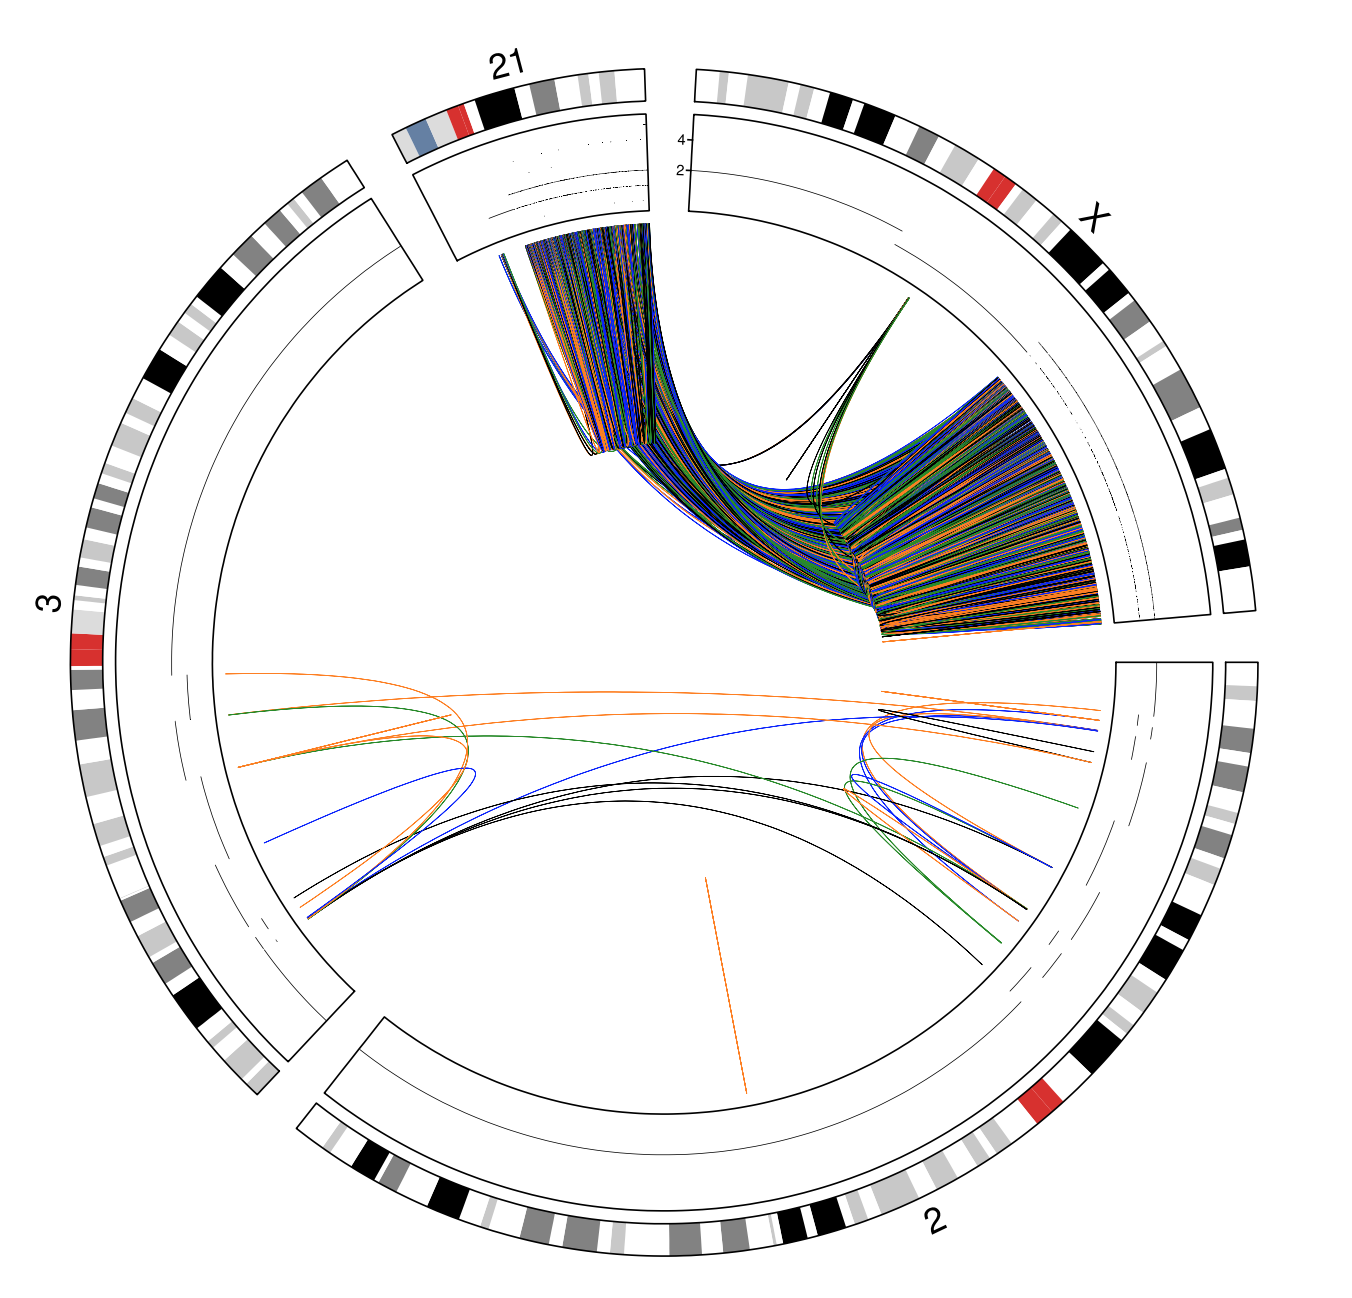
\includegraphics[width=9cm,height=9cm]{2939_massive.png}
\caption{Evidence of two massive multichromosomal chromothripsis events involving 
chromosomes 21-X and 2-3 detected in a kidney renal cell carcinoma tumor in patient DO17373 (TCGA-CJ-5681).}
\end{center}
\end{figure}


Shatterseek requires the SV data to be stored in a data.frame with the following columns: 
\begin{itemize}
\item chrom1 (character): chromosome for the first of the two breakpoints composing each SV
\item pos1 (character): position for the first breakpoint
\item chrom2 (character): chromosome for the second breakpoint composing each SV
\item pos2 (character): position for the second breakpoint
\item SVtype (character): type of SV, encoded as: DEL (deletion-like; +/-), DUP (duplication-like; -/+),
h2hINV (head-to-head inversion; +/+), and t2tINV (tail-to-tail inversion; -/-).
\item strand1
\item strand2
\end{itemize}
Chromosomes are expected to be in Ensembl chromosome notation, i.e. NOT contain the prefix "chr".\\
\begin{knitrout}
\definecolor{shadecolor}{rgb}{0.969, 0.969, 0.969}\color{fgcolor}\begin{kframe}
\begin{alltt}
\hlkwd{head}\hlstd{(SV_DO17373)}
\end{alltt}
\begin{verbatim}
##   chrom1    start1      end1 chrom2   start2     end2       sv_id
## 1      1 142618685 142618686     21 21708092 21708093 SVMERGE1159
## 2      1 142623413 142623414     21 25233137 25233138  SVMERGE269
## 3      1 142639910 142639911     21 33703275 33703276  SVMERGE127
## 4      1 143536371 143536372     21 29698088 29698089 SVMERGE1343
## 5     11   8540384   8540385     11  8541772  8541773   SVMERGE55
## 6     14  61896353  61896354     14 62061595 62061596 SVMERGE1006
##   pe_support strand1 strand2 svclass                    svmethod
## 1         18       +       -     TRA               SNOWMAN_DELLY
## 2         50       -       -     TRA       SNOWMAN_dRANGER_DELLY
## 3         34       +       -     TRA             SNOWMAN_dRANGER
## 4         39       -       +     TRA             SNOWMAN_dRANGER
## 5         37       +       -     DEL         SNOWMAN_BRASS_DELLY
## 6        111       -       +     DUP SNOWMAN_BRASS_dRANGER_DELLY
\end{verbatim}
\end{kframe}
\end{knitrout}



% SV_sample = "9ae0744a-9bc1-4cd7-b7cf-c6569ed9e4aa.pcawg_consensus_1.6.161022.somatic.sv.bedpe"
% SV.sample <- read.csv(SV_sample,sep="\t",header=T,stringsAsFactors=F)
% saveRDS(SV.sample,file="SV_9e07.rds")
% @

%%%<<echo=TRUE,warning=FALSE,message=FALSE,eval=TRUE,tidy=TRUE,render=T,fig.align='center',fig.cap="CV",out.width='8cm'>>=

Please remember that Shatterseek only considers chromosomes 1-22 and X.
Thus, make sure that the SVs comprised in your input data only correspond to these chromosomes.
The SV data is loaded into an object of class "SV", using the function {\it SVs}:

% # chrs <- c("1","2","3","4","5","6","7","8","9","10","11","12",
% #          "13","14","15","16","17","18","19","20","21","22","X")
% # SV.sample <- SV.sample[which(SV.sample$chrom1 %in% chrs & SV.sample$chrom2 %in% chrs),]

\begin{knitrout}
\definecolor{shadecolor}{rgb}{0.969, 0.969, 0.969}\color{fgcolor}\begin{kframe}
\begin{alltt}
\hlstd{SV_data} \hlkwb{<-} \hlkwd{SVs}\hlstd{(}\hlkwc{chrom1}\hlstd{=}\hlkwd{as.character}\hlstd{(SV_DO17373}\hlopt{$}\hlstd{chrom1),}
                \hlkwc{pos1}\hlstd{=}\hlkwd{as.numeric}\hlstd{(SV_DO17373}\hlopt{$}\hlstd{start1),}
                \hlkwc{chrom2}\hlstd{=}\hlkwd{as.character}\hlstd{(SV_DO17373}\hlopt{$}\hlstd{chrom2),}
                \hlkwc{pos2}\hlstd{=}\hlkwd{as.numeric}\hlstd{(SV_DO17373}\hlopt{$}\hlstd{end2),}
                \hlkwc{SVtype}\hlstd{=}\hlkwd{as.character}\hlstd{(SV_DO17373}\hlopt{$}\hlstd{svclass),}
                \hlkwc{strand1}\hlstd{=}\hlkwd{as.character}\hlstd{(SV_DO17373}\hlopt{$}\hlstd{strand1),}
                \hlkwc{strand2}\hlstd{=}\hlkwd{as.character}\hlstd{(SV_DO17373}\hlopt{$}\hlstd{strand2))}
\end{alltt}
\end{kframe}
\end{knitrout}


Shatterseek requires the CN to be in the following format:
(i)
\begin{itemize}
\item chrom (character): chromosome (also in Ensembl notation)
\item start (character): start position for the CN segment
\item end (character): end position for the CN segment
\item CN (character): absolute copy number value
\end{itemize}
\begin{knitrout}
\definecolor{shadecolor}{rgb}{0.969, 0.969, 0.969}\color{fgcolor}\begin{kframe}
\begin{alltt}
\hlkwd{head}\hlstd{(SCNA_DO17373)}
\end{alltt}
\begin{verbatim}
##   chromosome    start       end total_cn
## 1          1        1 249250620        2
## 3          2    20016  11969465        2
## 4          2 11969466  14420187        1
## 5          2 14420188  16916033        2
## 6          2 16916034  16937471        1
## 7          2 16937472  17054487        2
\end{verbatim}
\end{kframe}
\end{knitrout}

The CN data is  loaded into an object of class "CNVsegs", using the function {\it CNVsegs}:

% # <<echo=TRUE,results='hide',warning=FALSE,message=FALSE,eval=FALSE,tidy=TRUE,render=T>>=
% # CNV = "9ae0744a-9bc1-4cd7-b7cf-c6569ed9e4aa.consensus.20170119.somatic.cna.annotated.txt"
% # segSample <- read.csv(CNV,header=T,sep="\t",stringsAsFactors=F)
% # segSample$chromosome <- gsub("chr","",segSample$chromosome)
% # segSample <- segSample[which(segSample$chromosome != "Y"),]
% # @
% # 
% # <<echo=FALSE,results='hide',warning=FALSE,message=FALSE,eval=FALSE,tidy=TRUE,render=T>>=
% # ########
% # dd <- segSample[,c(1,2,3,4)]
% # dd$total_cn[dd$total_cn == 0] <- 15000
% # dd$total_cn[is.na(dd$total_cn)] <- 0
% # library(GenomicRanges)
% # dd <- as(dd,"GRanges")
% # cov <- coverage(dd,weight = dd$total_cn)
% # dd1 <- as(cov,"GRanges")
% # dd1 <- as.data.frame(dd1)
% # dd1 <- dd1[dd1$score !=0,]
% # head(dd1)
% # dd1 = dd1[,c(1,2,3,6)]
% # names(dd1) <- names(segSample)[1:4]
% # dd1$total_cn[dd1$total_cn == 15000] <- 0
% # #######
% # segSample = dd1
% # saveRDS(segSample,file="CNV_9e07.rds")
% # @

\begin{knitrout}
\definecolor{shadecolor}{rgb}{0.969, 0.969, 0.969}\color{fgcolor}\begin{kframe}
\begin{alltt}
\hlstd{CN_data} \hlkwb{<-} \hlkwd{CNVsegs}\hlstd{(}\hlkwc{chrom}\hlstd{=}\hlkwd{as.character}\hlstd{(SCNA_DO17373}\hlopt{$}\hlstd{chromosome),}
                     \hlkwc{start}\hlstd{=SCNA_DO17373}\hlopt{$}\hlstd{start,}
                     \hlkwc{end}\hlstd{=SCNA_DO17373}\hlopt{$}\hlstd{end,}
                     \hlkwc{total_cn}\hlstd{=SCNA_DO17373}\hlopt{$}\hlstd{total_cn)}
\end{alltt}
\end{kframe}
\end{knitrout}


%%\section{Identifying clusters of interleaved SVs using the function {\it shatterseek}}
Once the input data has been loaded, we proceed to run the main function of the package,
namely {\it shatterseek}.
This function runs the code to detect clusters of interleaved SVs, 
and subsequently evaluates each candidate chromothripsis region for
the statistical criteria described above.
%library(GenomicRanges)
\begin{knitrout}
\definecolor{shadecolor}{rgb}{0.969, 0.969, 0.969}\color{fgcolor}\begin{kframe}
\begin{alltt}
\hlkwd{library}\hlstd{(shatterSeek)}
\hlstd{start_time} \hlkwb{<-} \hlkwd{Sys.time}\hlstd{()}
\hlstd{chromothripsis} \hlkwb{<-} \hlkwd{shatterseek}\hlstd{(}\hlkwc{SV.sample}\hlstd{=SV_data,} \hlkwc{seg.sample}\hlstd{=CN_data)}
\end{alltt}
\begin{verbatim}
## Running..
## 
## 
## Evaluating the statistical criteria
## Successfully finished!
\end{verbatim}
\begin{alltt}
\hlstd{end_time} \hlkwb{<-} \hlkwd{Sys.time}\hlstd{()}
\hlkwd{print}\hlstd{(}\hlkwd{paste0}\hlstd{(}\hlstr{"Running time (s): "}\hlstd{,end_time} \hlopt{-} \hlstd{start_time))}
\end{alltt}
\begin{verbatim}
## [1] "Running time (s): 17.0460901260376"
\end{verbatim}
\begin{alltt}
\hlkwd{print}\hlstd{(}\hlkwd{head}\hlstd{(chromothripsis}\hlopt{@}\hlkwc{chromSummary}\hlstd{))}
\end{alltt}
\begin{verbatim}
##   chrom     start       end number_DEL number_DUP number_h2hINV
## 1     1        NA        NA          0          0             0
## 2     2  11969466  75460870          3          3             2
## 3     3  20704347  85709275          2          1             1
## 4     4        NA        NA          0          0             0
## 5     5 140129029 171935828          0          2             0
## 6     6        NA        NA          0          0             0
##   number_t2tINV number_TRA clusterSize_including_TRA number_SVs_sample
## 1             0          0                         0              1426
## 2             0          7                        15              1426
## 3             0          6                        10              1426
## 4             0          0                         0              1426
## 5             0          0                         2              1426
## 6             0          0                         0              1426
##   number_CNV_segments pval_fragment_joins chr_breakpoint_enrichment
## 1                  NA                  NA              8.612611e-17
## 2                  13           0.8653370              2.949495e-08
## 3                  14           0.5724067              1.185413e-07
## 4                  NA                  NA              1.852862e-17
## 5                   1           0.1116102              6.729654e-15
## 6                  NA                  NA              3.277719e-14
##   pval_exp_chr pval_exp_cluster
## 1           NA               NA
## 2 1.606883e-07     0.000000e+00
## 3 0.000000e+00     4.466794e-10
## 4           NA               NA
## 5           NA               NA
## 6           NA               NA
##   max_number_oscillating_CN_segments_2_states
## 1                                          NA
## 2                                          11
## 3                                          12
## 4                                          NA
## 5                                          NA
## 6                                          NA
##   max_number_oscillating_CN_segments_2_states_3states
## 1                                                  NA
## 2                                                  11
## 3                                                  12
## 4                                                  NA
## 5                                                  NA
## 6                                                  NA
##   number_CN_segments_chr max_number_oscillating_CN_segments_2_states_chr
## 1                     NA                                              NA
## 2                     13                                              13
## 3                     13                                              13
## 4                     NA                                              NA
## 5                     NA                                              NA
## 6                     NA                                              NA
##   max_number_oscillating_CN_segments_3_states_chr number_CN_segments
## 1                                              NA                 NA
## 2                                              13                 11
## 3                                              13                 12
## 4                                              NA                 NA
## 5                                              NA                 NA
## 6                                              NA                 NA
##   inter_number_DEL inter_number_h2hINV inter_number_t2tINV
## 1                0                   0                   0
## 2                4                   2                   3
## 3                4                   3                   4
## 4                0                   0                   0
## 5                0                   0                   0
## 6                0                   0                   0
##   inter_number_TRA inter_number_DUP inter_pval_fragment_joins
## 1                0                0                        NA
## 2                7                2                 0.8012520
## 3                6                3                 0.9626925
## 4                0                0                        NA
## 5                0                0                        NA
## 6                0                0                        NA
##   inter_other_chroms inter_other_chroms_coords_all
## 1                                                 
## 2                  3          3:20704347-85709275;
## 3                  2          2:11969466-75460870;
## 4                                                 
## 5                                                 
## 6
\end{verbatim}
\end{kframe}
\end{knitrout}
The 'clusterSize' column indicates the size of the largest cluster of interleaved SVs detected per chromosome.

\begin{knitrout}
\definecolor{shadecolor}{rgb}{0.969, 0.969, 0.969}\color{fgcolor}\begin{kframe}
\begin{alltt}
\hlcom{#chromothripsis@chromSummary }
\hlkwd{detach}\hlstd{(}\hlstr{"package:shatterSeek"}\hlstd{,} \hlkwc{unload}\hlstd{=}\hlnum{TRUE}\hlstd{)}
\hlkwd{library}\hlstd{(shatterSeek)}
\hlcom{#o = statistical_criteria(chromothripsis)}
\end{alltt}
\end{kframe}
\end{knitrout}


The function {\it shatterseek} returns a list containing two objects:

\begin{itemize}
\item sd


%%% SUMMARY
\item chromSummary: a data.frame containing the results for all statistical criteria described above and additional information. 
Each row corresponds to a chromosome (i.e., 1-22, and X), whereas the columns contain the following information:
\begin{itemize}
\item sdf
\item
\item
\item
\item
\item
\end{itemize}
\end{itemize}





\section{Visualization of chromothripsis regions}

\begin{knitrout}
\definecolor{shadecolor}{rgb}{0.969, 0.969, 0.969}\color{fgcolor}\begin{kframe}
\begin{alltt}
\hlkwd{library}\hlstd{(gridExtra)}
\hlstd{plots_chr3} \hlkwb{=} \hlkwd{plot_chromothripsis}\hlstd{(}\hlkwc{shatterSeek_output} \hlstd{= chromothripsis,}\hlkwc{chr} \hlstd{=} \hlstr{"3"}\hlstd{)}
\hlcom{#grid.arrange(plots_chr3[[1]],plots_chr3[[2]],plots_chr3[[3]],plots_chr3[[4]],nrow=4,ncol=1,heights=c(0.2,.4,.55,.25))}
\hlstd{plot_chr3} \hlkwb{=} \hlkwd{arrangeGrob}\hlstd{(plots_chr3[[}\hlnum{1}\hlstd{]],plots_chr3[[}\hlnum{2}\hlstd{]],plots_chr3[[}\hlnum{3}\hlstd{]],plots_chr3[[}\hlnum{4}\hlstd{]],}
                        \hlkwc{nrow}\hlstd{=}\hlnum{4}\hlstd{,}\hlkwc{ncol}\hlstd{=}\hlnum{1}\hlstd{,}\hlkwc{heights}\hlstd{=}\hlkwd{c}\hlstd{(}\hlnum{0.2}\hlstd{,}\hlnum{.4}\hlstd{,}\hlnum{.4}\hlstd{,}\hlnum{.25}\hlstd{))}

\hlstd{plots_chr2} \hlkwb{=} \hlkwd{plot_chromothripsis}\hlstd{(}\hlkwc{shatterSeek_output} \hlstd{= chromothripsis,}\hlkwc{chr} \hlstd{=} \hlstr{"2"}\hlstd{)}
\hlstd{plot_chr2} \hlkwb{=} \hlkwd{arrangeGrob}\hlstd{(plots_chr2[[}\hlnum{1}\hlstd{]],plots_chr2[[}\hlnum{2}\hlstd{]],plots_chr2[[}\hlnum{3}\hlstd{]],plots_chr2[[}\hlnum{4}\hlstd{]],}
                        \hlkwc{nrow}\hlstd{=}\hlnum{4}\hlstd{,}\hlkwc{ncol}\hlstd{=}\hlnum{1}\hlstd{,}\hlkwc{heights}\hlstd{=}\hlkwd{c}\hlstd{(}\hlnum{0.2}\hlstd{,}\hlnum{.4}\hlstd{,}\hlnum{.4}\hlstd{,}\hlnum{.25}\hlstd{))}

\hlstd{plots_chr21} \hlkwb{=} \hlkwd{plot_chromothripsis}\hlstd{(}\hlkwc{shatterSeek_output} \hlstd{= chromothripsis,}\hlkwc{chr} \hlstd{=} \hlstr{"21"}\hlstd{)}
\hlstd{plot_chr21} \hlkwb{=} \hlkwd{arrangeGrob}\hlstd{(plots_chr21[[}\hlnum{1}\hlstd{]],plots_chr21[[}\hlnum{2}\hlstd{]],plots_chr21[[}\hlnum{3}\hlstd{]],plots_chr21[[}\hlnum{4}\hlstd{]],}
                        \hlkwc{nrow}\hlstd{=}\hlnum{4}\hlstd{,}\hlkwc{ncol}\hlstd{=}\hlnum{1}\hlstd{,}\hlkwc{heights}\hlstd{=}\hlkwd{c}\hlstd{(}\hlnum{0.2}\hlstd{,}\hlnum{.4}\hlstd{,}\hlnum{.4}\hlstd{,}\hlnum{.25}\hlstd{))}

\hlstd{plots_chrX} \hlkwb{=} \hlkwd{plot_chromothripsis}\hlstd{(}\hlkwc{shatterSeek_output} \hlstd{= chromothripsis,}\hlkwc{chr} \hlstd{=} \hlstr{"X"}\hlstd{)}
\end{alltt}


{\ttfamily\noindent\bfseries\color{errorcolor}{\#\# Error: evaluation nested too deeply: infinite recursion / options(expressions=)?}}\begin{alltt}
\hlstd{plot_chrX} \hlkwb{=} \hlkwd{arrangeGrob}\hlstd{(plots_chrX[[}\hlnum{1}\hlstd{]],plots_chrX[[}\hlnum{2}\hlstd{]],plots_chrX[[}\hlnum{3}\hlstd{]],plots_chrX[[}\hlnum{4}\hlstd{]],}
                        \hlkwc{nrow}\hlstd{=}\hlnum{4}\hlstd{,}\hlkwc{ncol}\hlstd{=}\hlnum{1}\hlstd{,}\hlkwc{heights}\hlstd{=}\hlkwd{c}\hlstd{(}\hlnum{0.2}\hlstd{,}\hlnum{.4}\hlstd{,}\hlnum{.4}\hlstd{,}\hlnum{.25}\hlstd{))}
\end{alltt}


{\ttfamily\noindent\bfseries\color{errorcolor}{\#\# Error in arrangeGrob(plots\_chrX[[1]], plots\_chrX[[2]], plots\_chrX[[3]], : object 'plots\_chrX' not found}}\begin{alltt}
\hlkwd{grid.arrange}\hlstd{(plot_chr2,plot_chr3,plot_chr21,plot_chrX,}\hlkwc{ncol}\hlstd{=}\hlnum{2}\hlstd{,}\hlkwc{nrow}\hlstd{=}\hlnum{2}\hlstd{,}\hlkwc{heights}\hlstd{=}\hlkwd{c}\hlstd{(}\hlnum{.5}\hlstd{,}\hlnum{.5}\hlstd{),}\hlkwc{widths}\hlstd{=}\hlkwd{c}\hlstd{(}\hlnum{.5}\hlstd{,}\hlnum{.5}\hlstd{))}
\end{alltt}


{\ttfamily\noindent\bfseries\color{errorcolor}{\#\# Error in arrangeGrob(...): object 'plot\_chrX' not found}}\end{kframe}
\end{knitrout}


arrangeGrob(plots[[1]],plots[[2]],plots[[3]],plots[[4]],nrow=4,ncol=1,heights=c(0.2,.4,.55,.25))

\section{Visualization of multichromosomal chromothripsis events}


\section{Bibliography}
\printbibliography
\end{document}


